\chapter{Implementation}
\label{chap:impl}

\section{Jasmin language server}

This section presents the implementation of a Language Server Protocol (LSP)
interface for the Jasmin programming language, developed in OCaml. The server
directly integrates with Jasmin's compiler frontend, utilizing its existing type
system and AST representation to provide language features through LSP
communication. 

A reference Neovim client configuration demonstrates practical integration,
showcasing real-time static analysis and editor tooling capabilities while
maintaining consistency with the compiler's behavior. 

\subsection{Implementation details}
\label{impl:implementation-details}

The language server's core functionality is implemented in pure functions where
possible in the request handler components. This design choice significantly
simplifies both debugging and future extensions to the system. OCaml's advanced
type system provides benefits in this implementation, enabling compile-time
verification of complex invariants.

Let us proceed with the RPC server. The RPC server architecture employs a state
machine model with three distinct states: $Uninitialized$, $Running$, and
$Stopped$, as presented in Listing~\ref{lst:lsp-state-machine}. 

\begin{lstlisting}[
  caption          = {Main server loop}, 
  label            = {lst:lsp-state-machine},
  language         = {caml},
  numbers=left,
  backgroundcolor=\color{white},   % choose the background color
  basicstyle=\footnotesize,        % size of fonts used for the code
  breaklines=true,                 % automatic line breaking only at whitespace
  captionpos=b,                    % sets the caption-position to bottom
  commentstyle=\color{mygreen},    % comment style
  escapeinside={\%*}{*)},          % if you want to add LaTeX within your code
  keywordstyle=\color{blue},       % keyword style
  float
  ]
let start (server : Rpc_server.t) =
  let rec rpc_loop server =
    match server.state with
    | State.Stopped -> 
      Logs.info (fun m -> m "Server stopped");
      Lwt.return_unit;
    | _ -> (
      let%lwt client_msg = Utils.read () in
      match client_msg with
      | Some msg -> (
        let%lwt server = 
          let server, reply_result = 
          Message_handler.handle_message server msg
        in Lwt.dont_wait
          (fun () -> Utils.send reply_result)
          (notify_and_log_error_sync "Error");
        Lwt.return server
      in rpc_loop server
      )
      | None -> 
        Logs.debug (fun m -> m "Client disconnected");
        Lwt.return_unit
    )
    in rpc_loop server
\end{lstlisting}

In the $Uninitialized$ state, the server process has started but has not yet
established any client connections.  The transition to the $Running$ state
occurs when processing the client's \texttt{initialize} request, which triggers
several critical initialization procedures. These include setting up the
document storage system (implemented as an in-memory key-value store tracking
open files) and preparing various language service components, ending the
initialization process with the server response containing supported
capabilities.

Listing~\ref{lst:ls-supported-features} features the part of the initialization 
routine, which at the end creates (Listing~\ref{lst:ls-supported-features}, line
3) the \texttt{capabilities} variable representing language server supported
capabilities with some modifiers.

The $Running$ state maintains strict operational constraints, with only one
possible state transition --- to $Stopped$. This transition occurs under two
conditions: either when encountering unrecoverable errors (e.g. broken
communication pipe) or when processing a client \texttt{shutdown} request, which
gracefully terminates the language server.

Main server loop is implemented as the recursive call to the \texttt{rpc\_loop}
function (Listing~\ref{lst:lsp-state-machine}, line 2). During the loop
execution, the function matches the server state, and if the server is stopped,
it does not process client messages.  In other case
(Listing~\ref{lst:lsp-state-machine}, line 7), it starts client message handling
in a separate \texttt{lwt} thread, so the main thread can continue looping. This
is possible, since LSP designed in a way, that allows client to make requests
without waiting for server to respond before making a new one.

When the RPC server accepts the client JSON-RPC message, the server passes message to the
corresponding message handler, as shown in Listing~\ref{lst:message-handlers}. 
On line $3$ starts the pattern matching on the received JSON-RPC message, and during this 
matching, the server can process either LSP request, or LSP notification. In case (on line 13) 
some other LSP message was sent to the language server, nothing happens.

\begin{lstlisting}[
  caption          = {Message handlers}, 
  label            = {lst:message-handlers},
  language         = {caml},
  numbers=left,
  backgroundcolor=\color{white},   % choose the background color
  basicstyle=\footnotesize,        % size of fonts used for the code
  breaklines=true,                 % automatic line breaking only at whitespace
  captionpos=b,                    % sets the caption-position to bottom
  commentstyle=\color{mygreen},    % comment style
  escapeinside={\%*}{*)},          % if you want to add LaTeX within your code
  keywordstyle=\color{blue},       % keyword style
  float
  ]
let handle_message (server : Rpc_server.t) (msg : Packet.t) =
  Logs.debug (fun m -> m "handling message");
  match msg with 
  | Request req -> (
    Logs.debug (fun m -> m "handling request");
    on_request server req
  )
  | Notification notification -> (
    Logs.debug (fun m -> m "handling notification");
    let server, reply = handle_notification server notification in
    in server, reply
  )
  | _ -> (
    Logs.debug (fun m -> m "unknown message"); 
    server, msg
  )
\end{lstlisting}

Logging is performed into the separate configurable file, which allows for more 
convenient debugging. This implementation divides all logging messages into three
categories: debug, informational and error. Listing~\ref{lst:logging-setup} contains 
function which creates a file on the host file system with correct permissions and 
sets up logging reporter with debug log level.

\begin{lstlisting}[
  caption          = {Logging set up function}, 
  label            = {lst:logging-setup},
  language         = {caml},
  numbers=left,
  backgroundcolor=\color{white},   % choose the background color
  basicstyle=\footnotesize,        % size of fonts used for the code
  breaklines=true,                 % automatic line breaking only at whitespace
  captionpos=b,                    % sets the caption-position to bottom
  commentstyle=\color{mygreen},    % comment style
  escapeinside={\%*}{*)},          % if you want to add LaTeX within your code
  keywordstyle=\color{blue},       % keyword style
  float
  ]
let setup_logging_to_file filename =
  let file_formatter = 
    let oc = open_out_gen [Open_append;Open_trunc;Open_creat] 0o600 filename in
    Format.formatter_of_out_channel oc
  in
  
  let reporter = Logs_fmt.reporter ~dst:file_formatter () in
  
  Logs.set_reporter reporter;
  Logs.set_level (Some Logs.Debug);
  ()
\end{lstlisting}

Our language server implementation is designed to run as a standalone binary 
which communicates with the client via process stdin and stdout.

\subsection{Features}

Currently, language server supports the features specified below.

\subsubsection*{Real-time code diagnostics}


\label{impl:code-diagnostics}

Real-time code diagnostics is a vital feature in software development
environments, as it enables programmers to identify type and syntax errors in
the editing phase without executing the compiler. 

In our implementation, the code diagnostics process is executed within a
separate thread, triggered whenever the user saves the file they are working on,
processing the entire modified content. 

As illustrated in Listing~\ref{lst:ls-supported-features}, specifically on line
9, our language server supports the \texttt{Full} synchronization kind, meaning
that when the user saves or makes changes in the file, on each change, the whole
contents of the file is sent to the language server. In ideal case, language
server should accept the incremental changes, but this is not currently
supported, and probably will require some modifications to the compiler's source
code itself, since the compiler does not expose an API for incremental parsing.

\begin{lstlisting}[
  caption          = {Language server supported features}, 
  label            = {lst:ls-supported-features},
  language         = {caml},
  numbers=left,
  backgroundcolor=\color{white},   % choose the background color
  basicstyle=\footnotesize,        % size of fonts used for the code
  breaklines=true,                 % automatic line breaking only at whitespace
  captionpos=b,                    % sets the caption-position to bottom
  commentstyle=\color{mygreen},    % comment style
  escapeinside={\%*}{*)},          % if you want to add LaTeX within your code
  keywordstyle=\color{blue},       % keyword style
  float
  ]
let on_request (server : Rpc_server.t) (_params : InitializeParams.t) =
  ...
  let capabilities = 
    ServerCapabilities.create
    ~textDocumentSync:
      ( `TextDocumentSyncOptions
        (TextDocumentSyncOptions.create
          ~openClose:true
          ~change:TextDocumentSyncKind.Full
          ()
        )
      )
    ~workspace:
      (ServerCapabilities.create_workspace
         ~workspaceFolders:
           (WorkspaceFoldersServerCapabilities.create ~supported:true
              ~changeNotifications:(`Bool true) ())
         ())
    ~documentHighlightProvider:(`Bool true)
    ~definitionProvider:(`Bool true)
    ~hoverProvider:(`Bool true)
    ()
  in
  let serverInfo =
    InitializeResult.create_serverInfo ~name: "jasmin-lsp" ~version:"0.0.1" () in
  let init = 
    InitializeResult.create ~capabilities ~serverInfo () in
  let server = 
    {
      internal_state = new_internal_state;
      state = Rpc_server.State.Running
    }
  in server, init
\end{lstlisting}

The code diagnostics works in two distinct phases to provide comprehensive
feedback to the user. In the first phase, the language server attempts to parse
the source code each time it detects a change.  Effective error notification is
crucial at this stage, as it alerts the user when the language server encounters
parsing errors. User notification implemented by sending a server notification
request to the client, including all parsing errors encountered, as depicted in
Figure~\ref{fig:parsing-error}, where the compiler could not parse the token
\texttt{tooo} and returned an error. 

\begin{figure}[hbt]
  \centering
  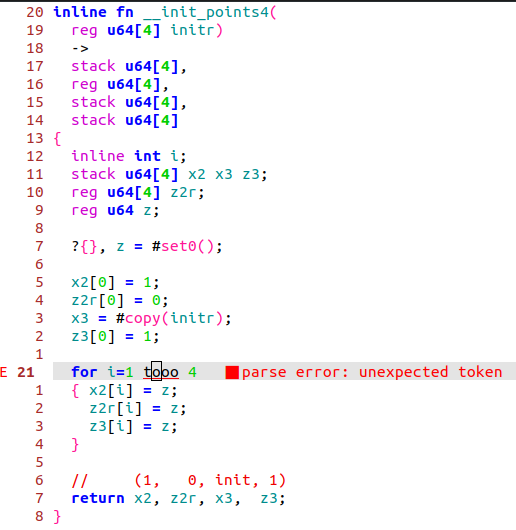
\includegraphics[width=0.95\textwidth]{figs/parse-error.png}
  \caption{Example of parsing error}
  \label{fig:parsing-error}
\end{figure} 

The second phase involves type inference, a critical process that requires the
language server to interface with the compiler API to obtain the typed AST.
During this phase, the compiler runs its internal typechecking algorithm that 
inferences all variable types and checks for illegal memory access Any errors
detected at this stage, such as type mismatches, are also communicated to the
user, as illustrated in Figure~\ref{fig:typing-error}, where one tries to assign
an array variable type (\texttt{stack u64[4]}) to an array element, where
elements are expected to be of type \texttt{u64}.

\begin{figure}[hbt]
  \centering
  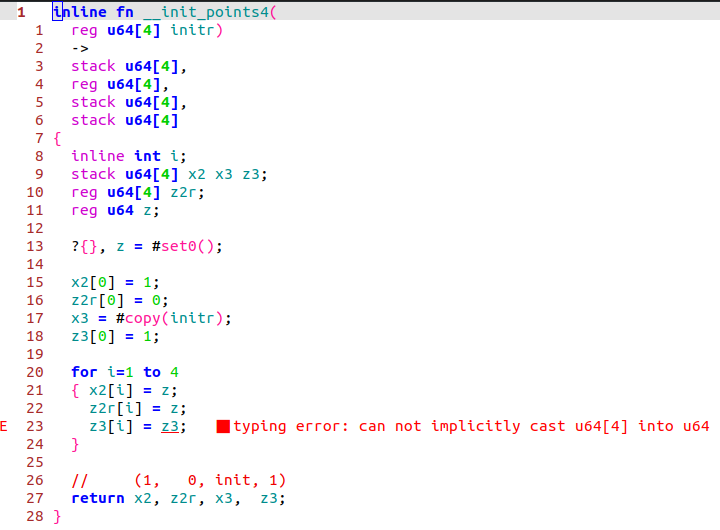
\includegraphics[width=0.95\textwidth]{figs/typing-error.png}
  \caption{Example of typing error}
  \label{fig:typing-error}
\end{figure} 

\subsection*{Symbol highlight}

The implementation of a symbol highlighting in our language server involves 
fetching additional info from the typed AST. Firstly, we locate relevant AST 
node in the internal representation that corresponds to the symbol under the 
cursor.

We then traverse the entire AST to identify all instances of that symbol with
the same identifier. This can easily be done, since Jasmin compiler assigns
unique identifiers to each symbol during the parsing and type inference stages.
These identifiers remain distinct across different compiler invocations,
ensuring that symbols are uniquely distinguished even if they share the same
name.

For instance, if a programmer redeclares a variable with an identical name
elsewhere in the code, the internal AST representation treats them as separate
entities, each with its own unique identifier. An example of symbol
highlighting, demonstrating this capability, is illustrated in
Figure~\ref{fig:symbol-highlight}, where the variable with the name \texttt{x2}
is highlighted in all its usages.

\begin{figure}[hbt]
  \centering
  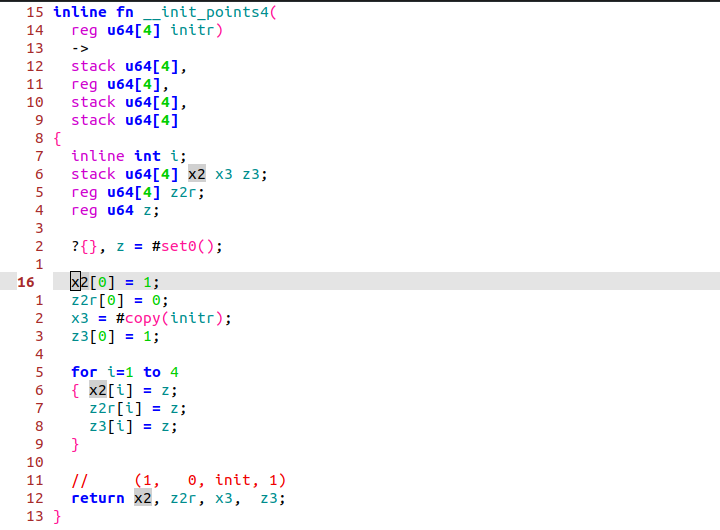
\includegraphics[width=0.95\textwidth]{figs/symbol-highlight.png}
  \caption{Example of symbol highlight}
  \label{fig:symbol-highlight}
\end{figure} 

\subsection*{Go to definition}

We implemented go to definition feature using the compiler's internal
representation of the symbol in the AST. Each node contains not only it's 
location in the project, but also, the definition location if applicable, making
the implementation of this feature rather easy.

\subsection*{Symbol type inference on hover (Type ascription)}

In developing the symbol type inference for our language server, we relied on
the Jasmin compiler's API to extract detailed information from the typed AST.
This API offers a set of functions for pretty printing, which enabled us to
directly access and format each symbol's type information. The primary goal of
implementing this LSP capability was to display the symbol's type to the user in
a clear, concise manner without undertaking additional operations on the type
data itself. By using the pretty-printing function, we could seamlessly present
this information as a hover tooltip, improving the coding experience.

As illustrated in Figure~\ref{fig:hover}, when the user hovers over the
variable \texttt{z}, the hover feature accurately displays its type as
\texttt{reg u64}. 

\begin{figure}[hbt]
  \centering
  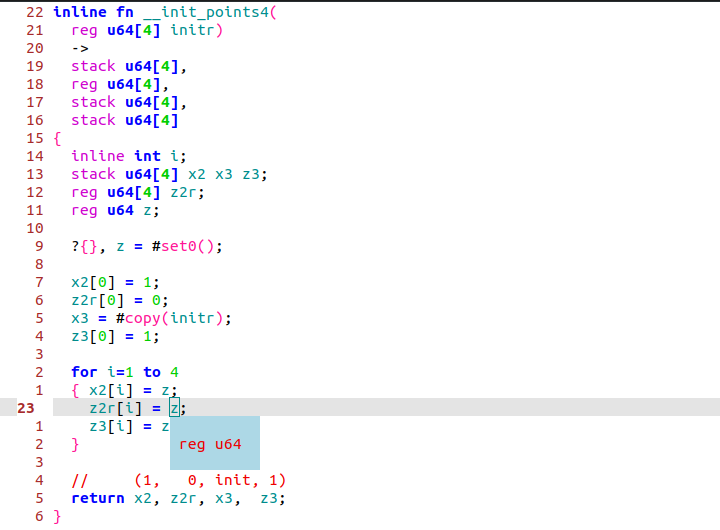
\includegraphics[width=0.9\textwidth]{figs/hover.png}
  \caption{Example of symbol type inference on hover}
  \label{fig:hover}
\end{figure} 


\section{Installation and configuration}

An example of how can one configure Neovim text editor to work with Jasmin 
language server is presented in Listing~\ref{lst:ls-nvim-config}. The configuration 
features the usage of filetype detection mechanism in Neovim, adding support 
for Jasmin (\texttt{.jazz}) files, as well as error handling logic, when the 
language server could not start for some reasons.

\begin{lstlisting}[
  caption={LS configuration example for neovim text editor}, 
  label={lst:ls-nvim-config},
  language         = {[5.2]Lua},
  numbers=left,
  backgroundcolor=\color{white},   % choose the background color
  basicstyle=\footnotesize,        % size of fonts used for the code
  breaklines=true,                 % automatic line breaking only at whitespace
  captionpos=b,                    % sets the caption-position to bottom
  commentstyle=\color{mygreen},    % comment style
  escapeinside={\%*}{*)},          % if you want to add LaTeX within your code
  keywordstyle=\color{blue},       % keyword style
  float
  ]
vim.filetype.add {
  extension = {
    jazz = 'jazz',
  },
}

local client = vim.lsp.start_client {
  name = 'jasmin-lsp',
  cmd = { '/path/to/jasmin-lsp/binary' },
  on_attach = vim.notify 'client initialized',
}

if not client then
  vim.notify 'client error'
end

vim.api.nvim_create_autocmd('FileType', {
  pattern = 'jazz',
  callback = function()
    vim.lsp.buf_attach_client(0, client)
  end,
}) 
\end{lstlisting}

As it was mentioned earlier in section~\ref{impl:implementation-details}, our
implementation is meant to run as a standalone binary, so, from the
Listing~\ref{lst:ls-nvim-config} (line 9) one can see that the text editor process
spawnes the language server proccess for further interaction.

\section{Tree-sitter support}

\subsection{Tree-sitter}
\label{impl:tree-sitter}

Tree-sitter \cite{tree-sitter} is a parsing system that can generate incremental
parsers for arbitrary user-defined grammars. It builds concrete syntax trees
that update in real-time as the source code changes, making it particularly
suitable for text editor tooling and language servers. Unlike traditional
parsers, tree-sitter handles incomplete code gracefully, enabling syntax
highlighting and code navigation.

\subsection{Implementation}

This section describes the implementation of the tree-sitter parser for the Jasmin
programming language.

In early stage of the language server development, we have implemented the
tree-sitter parser for the Jasmin programming language, as it provided syntax
highlighting, improving overall development experience.

As shown in Figure~\ref{fig:tree-sitter}, on the right hand side is the concrete
syntax tree (CST) for the code snippet, and the highlighted part on the left
hand side is the corresponding CST node of the source code. From this code 
snippet it can be seen, that the highlight queries give the flexibility in what 
parts of the concrete syntax tree we want to highlight.

\begin{figure}[hbt]
\centering
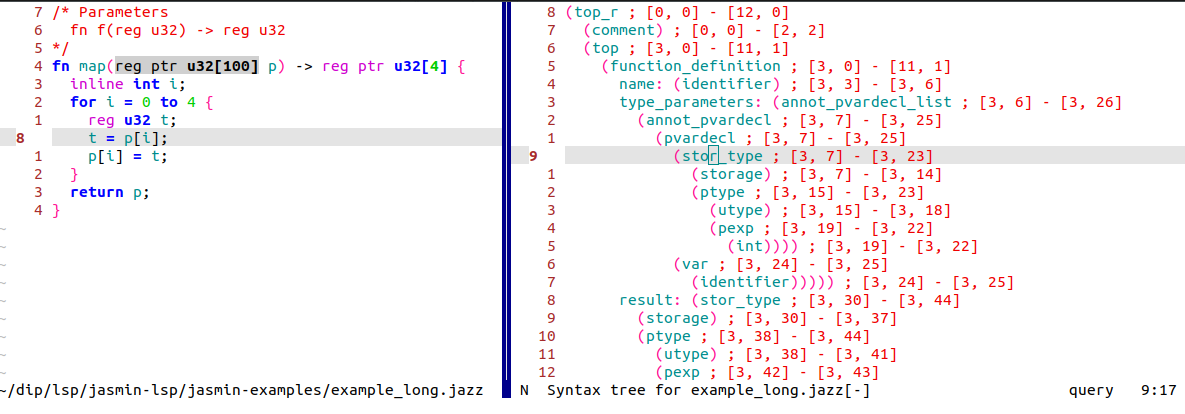
\includegraphics[width=\textwidth]{figs/tree-sitter-v4.png}

\caption{Tree-sitter highlight example}

\label{fig:tree-sitter}
\end{figure} 

The development process for a Tree-sitter parser typically involves two critical
phases: crafting a grammar for the target language and developing `highlight
queries' for the established grammar. Writing the grammar involves defining the
syntactic structure of the language, ensuring that all valid constructs are
accurately represented. This step is foundational, as it dictates how source
code is parsed into a concrete syntax tree (CST).

The Jasmin compiler utilizes Menhir~\cite{menhir} as its parser generator tool
for constructing the front-end component of the compiler. Menhir is a parser
generator for OCaml, known for its capacity to handle large and complex grammars
efficiently. It enables compiler developers to define the language's syntax in a
Backus-Naur Form (BNF)-like syntax, which simplifies expressing the grammatical
structure of programming languages. This high-level abstraction allows for more
readable and maintainable grammar specifications.

Once the grammar is formulated, Menhir generates the corresponding lexer and
parser from this definition. This automatic generation is crucial, as it
abstracts the underlying complexity of syntax analysis and reduces human errors.
Menhir's error error handling and support for advanced parsing techniques, such
as LR(1), further enhance the compiler's ability to provide meaningful syntax
error messages and efficient parsing routines.

Highlight queries are particularly important because Tree-sitter generates and
utilizes the CST without knowledge of the semantics represented by each node.
For example, the CST does not inherently distinguish between nodes representing
function identifiers and those representing user-defined types. By implementing
highlight queries, we can assign semantic meaning to specific CST nodes,
providing color-coded syntax highlighting that enhances code readability and
aids developers in quickly identifying code elements. 

\subsection{Installation and configuration}

Assuming that the user has the Jasmin file type supported in Neovim, they can
use the configuration presented in Listing~\ref{lst:tree-sitter-nvim-config} to
add tree-sitter support for the Jasmin programming language.

This configuration adds the tree-sitter mapping for the \texttt{jazz} filetye,
which represents the Jasmin language, specifying that the parser firstly must be
downloaded from the external github repository.

After modifying the configuration user must install the tree-sitter for the
Jasmin separately.

\begin{lstlisting}[
  caption={Tree-sitter configuration example for neovim text editor}, 
  label={lst:tree-sitter-nvim-config},
  language         = {[5.2]Lua},
  numbers=left,
  backgroundcolor=\color{white},   % choose the background color
  basicstyle=\footnotesize,        % size of fonts used for the code
  breaklines=true,                 % automatic line breaking only at whitespace
  captionpos=b,                    % sets the caption-position to bottom
  commentstyle=\color{mygreen},    % comment style
  escapeinside={\%*}{*)},          % if you want to add LaTeX within your code
  keywordstyle=\color{blue},       % keyword style
  float
  ]
local parser_config = require('nvim-treesitter.parsers').get_parser_configs()
parser_config.jasmin = {
  install_info = {
    url = 'https://github.com/y4cer/tree-sitter-jasmin',
    files = { 'src/parser.c' },
    generate_requires_npm = false,
    requires_generate_from_grammar = false,
  },
  filetype = 'jazz',
}
\end{lstlisting}
